% !TeX encoding = UTF-8
% !TeX spellcheck = en_GB
% !TeX root = mythesis.tex
\chapter{Edge-magneto-plasmon squeezing}

Le projet de squeezing

\begin{figure}[hptb]
	\begin{center}
		\begin{tabular}{c}
			 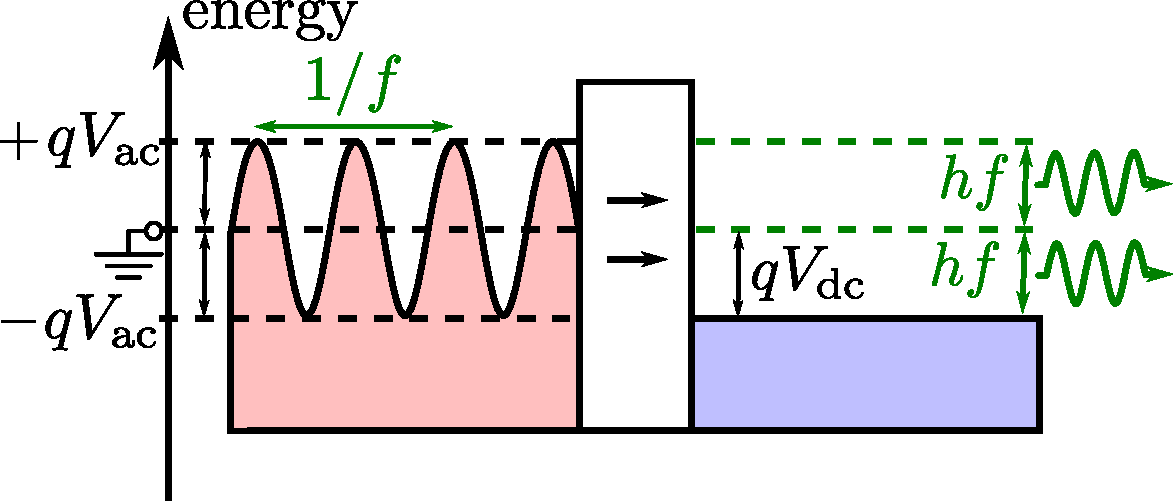
\includegraphics[width = 6.5 cm]{./chap3/noise_schematics}
		\end{tabular}
	\end{center}
	
	\caption{\textbf{title.}}
	\label{fig: squeezing principle schematics}
\end{figure}

\section{Experimental set-up}

In this section the electrical circuits used to perform the measurements are presented.
The measurements have been realized in two steps, the first measurement is the noise generated by the RF sinus voltage excitation, and the second measurement is the noise generated by the DC voltage excitation.
These two electrical circuits are drawn in figure Fig. \ref{fig: set-up chap 3}.

\begin{figure}
	\centering
	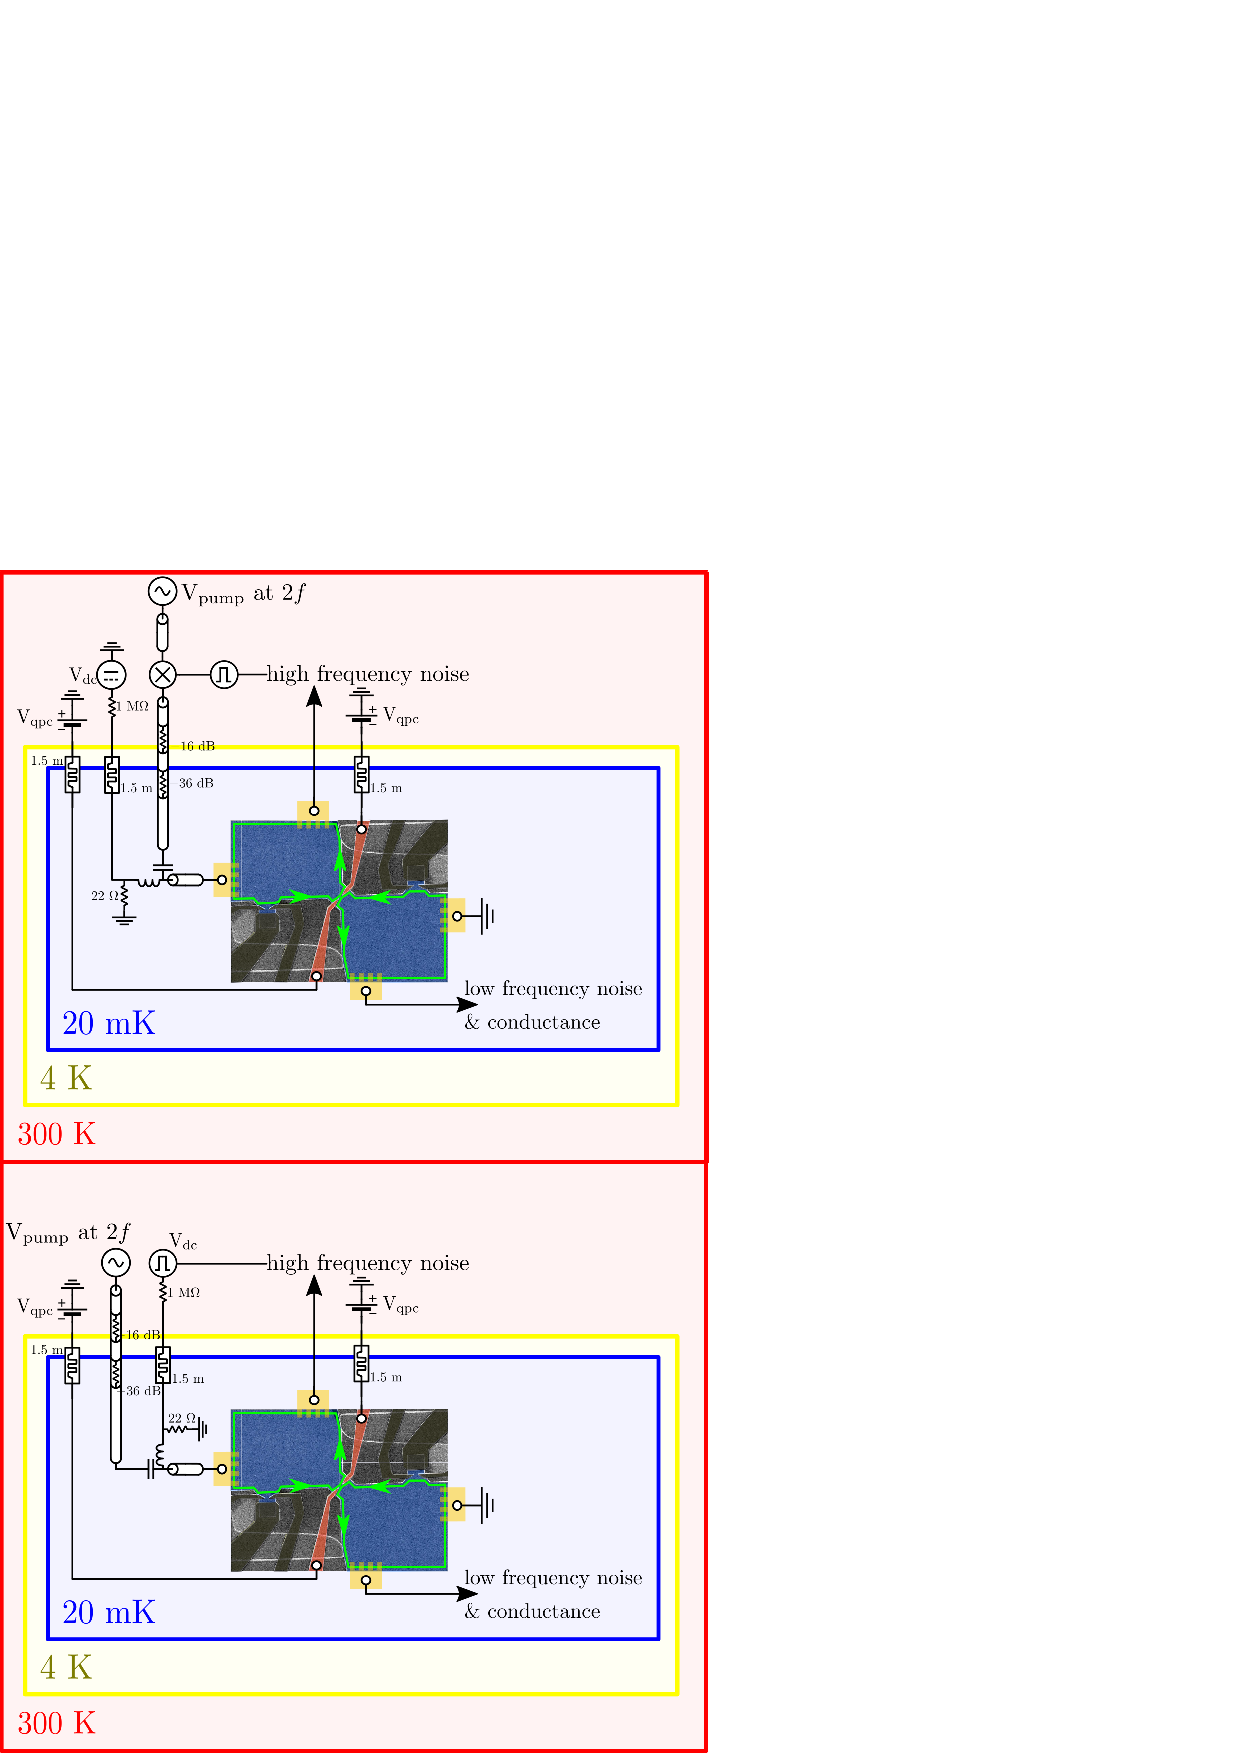
\includegraphics[width = 10cm]{./chap3/set-up_bruit_RF_pour_squeezing.pdf}
	\caption{\textbf{Electrical circuits for edge-magneto-plasmon squeezing measurement.} The circuit in the top panel is used to measure the high frequency noise of the pump sinus voltage $V_{\mathrm{pump}}$ at twice the measurement frequency $2f$. The pump voltage is modulated with a mixer by a square voltage at $\sim 230$ Hz included between $0$ V and $0.75$ V. The modulation signal is used in the RF noise measurement set-up represented in figure Fig. \ref{fig: le set-up chap2}. The pump voltage is added to a DC voltage with a bias tee at cold temperature. The circuit in the bottom panel enables to measure the high frequency noise of a DC voltage with the pump voltage. The square voltage at $\sim 230$ Hz is used for both the modulation and demodulation and to apply the DC voltage as it is included between $0$ V and $V_{\mathrm{dc}}$.}
	\label{fig: set-up chap 3}
\end{figure}

\subsection{Measurement of noise generated by the RF sinus voltage}

The top part of the figure Fig. \ref{fig: set-up chap 3} represents the circuit to measure the effect on the noise of the RF signal.
The measurement lines are not represented since they have been explained in the precedent chapters.
The low frequency noise is measured thanks to the circuit drawn in chapter 2, and the high frequency noise is measured thanks to the circuit drawn in chapter 1.
The high frequency measurement circuit uses a modulation of the source, which is done by a low frequency square voltage and a mixer.
The mixer is used as a switch for the RF sinus source as it is controlled by the low frequency square signal alternating between $0$ V and $0.75$ V.
After passing through the mixer, the RF sinus voltage, noted $V_{\mathrm{pump}}$, is attenuated and added to a DC voltage before exciting an edge-channel.
The DC voltage source is independent of the low frequency source generating the modulation signal, so the voltage $V_{\mathrm{DC}}$ is continuously applied on the edge-channel.
This set-up allows to measure the noise difference between two situations when both RF sinus voltage source and DC voltage source are turned on and when only DC voltage source is turned on.
This set-up access the excess high frequency noise of the voltage pump over the thermal noise when $V_{dc}$ is set at 0 V.

\subsection{Measurement of noise generated by the DC voltage}

The bottom part of the figure Fig. \ref{fig: set-up chap 3} is a drawing of the set-up used to probe how the variation of the voltage $V_{dc}$ affects the high frequency noise.
For this purpose the modulated signal is the DC Voltage $V_{dc}$, which is a square signal between 0 V and $V_{dc}$ produced by a low frequency function generator.
It is attenuated by a voltage divider and added to the RF sinus before its connection with an edge-channel.
In this set-up the RF sinus voltage is continuously generated, the high frequency noise measured is the difference of noise between both RF sinus and DC voltage are applied and only the noise of the RF sinus.
This connexion allows to measure the reduction of the high frequency noise compared to the noise of the RF sinus alone.

The two sources DC and RF are modulated separately because non-linearities of elements in the high frequency noise measurement chain.
These non-linearities generate strong parasitic signals in case of simultaneous modulation which blind the measurement.
The separated modulation cancel these parasitic and still allows to recover the total high frequency noise reduction compared to thermal noise by adding the two measurements.
Only the thermal noise is not measured but it is very close to vacuum noise because $\dfrac{hf}{k_{B}T} ...$, the thermal energy is too low to generate high frequency noise.

\section{Squeezed state evidence in quantum hall regime by high frequency noise measurement}

\subsection{Spectroscopy characterization of RF sinus excitation}

\begin{figure}[hptb]
	\begin{center}
		\begin{tabular}{c c c c}
			(a) & & (b) & \\
			& 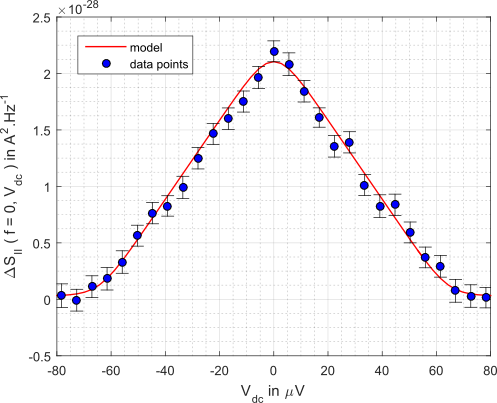
\includegraphics[width = 6.5 cm]{./chap3/LF_noise_pump_vs_V_dc} &
			& 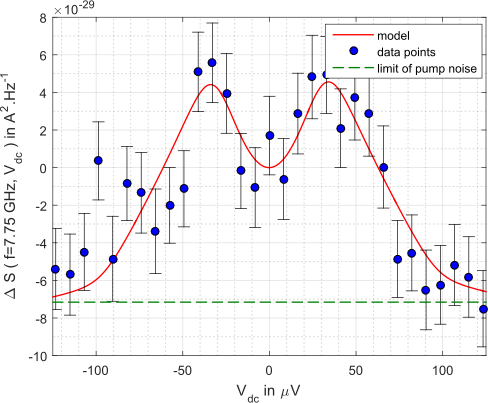
\includegraphics[width = 6.5 cm]{./chap3/RF_noise_pump_vs_V_dc}
		\end{tabular}
	\end{center}
	
	\caption{\textbf{Pump contribution to excess noise as a function of bias voltage.} \textbf{(a)} Low frequency noise difference between shot noise with the pump voltage and shot noise without pump $\Delta S_{II} = S_{II}\left(V_{\mathrm{ac}}\right) - S_{II}\left(V_{\mathrm{ac}}=0\right)$. \textbf{(b)} High frequency noise difference between noise with pump voltage and without pump voltage. For this measurement the high frequency measurement set-up of figure Fig. \ref{fig: le set-up chap2} is changed. The local oscillator, I-Q mixers, low pass filters, diodes, differential amplifiers, are replaced by a band pass filter around $f = 7.75$ GHz and a diode. With this change the magnitude of the total noise is measured instead of its real and imaginary part. The bias is still modulated so the value at $V_{dc} = 0$ is still substracted. The measured noise is then $\Delta\left|S_{II}\right|\left(V_{\mathrm{ac}}\right)-\Delta\left|S_{II}\right|\left(V_{\mathrm{ac} = 0}\right)$. And it tends the opposite of noise of the pump at large bias represented by the green dashed line. The models for both panels are computed thanks to the Wigner distribution of the pump.}
	\label{fig: noise pump vs Vdc}
\end{figure}

In the chapter ... the Wigner function of RF excitations is determined with low frequency noise measurements.
The control of the RF sinus voltage used in this chapter relies in part on the same measurements.
Only the first measurement of low frequency noise when both the RF source signal and the DC voltage bias are applied on the quantum point contact is performed.
The consistency between the model and the measurements gives the parameters of the RF sinus voltage.
In the panel (a) of figure \ref{fig: noise pump vs Vdc} the measurement is performed with a RF sinus voltage of frequency $f = 15.5$ GHz and an amplitude $V_{ac}$ around 38 $\upmu$V at the quantum point contact level.
The agreement between the model line and the data points confirms the values of amplitude and frequency of the RF sinus.

With this set-up we can performed the same kind of measurement by recording the high frequency noise instead of the low frequency one.
In this measurement we are interested in the magnitude of the noise, so the elements from the I-Q mixers to the differential amplifiers are replaced by a band pass filter around $f = 7.75$ GHz and a diode. 
The data points of obtained are plotted in the panel (b) of figure \ref{fig: noise pump vs Vdc}.
The noise without the RF voltage is subtracted to the noise from both RF and DC voltage to get the excess noise in the same way as the low frequency measurements.
The noise value at $V_{\mathrm{dc}} = 0$ V differs from the low frequency noise because the DC voltage is modulated in the high frequency set-up.
This modulation leads to a zero value of the measured excess noise at $V_{\mathrm{dc}} = 0$ V because it is automatically subtracted by the modulation.
The data points are consistent with numerical calculation in red line whose high $V_{\mathrm{dc}}$ limit is minus the high frequency noise of the RF sinus alone.
That limit is displayed on the graph by a green dashed line and will be directly measured in the next paragraph.
This second measurement adds an other indication of the amplitude and frequency of the RF sinus, and gives a first hint of the noise value added by the RF sinus. 

\subsection{High frequency noise of a RF sinus}

\begin{figure}[hptb]
	\begin{center}
		\begin{tabular}{c c c c}
			(a) & & (b) & \\
			& 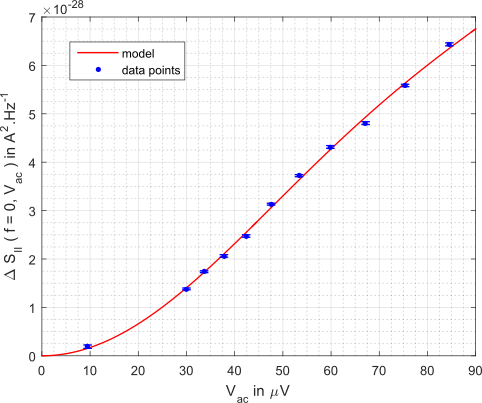
\includegraphics[width = 6.5 cm]{./chap3/LF_noise_vs_pump_amp} &
			& 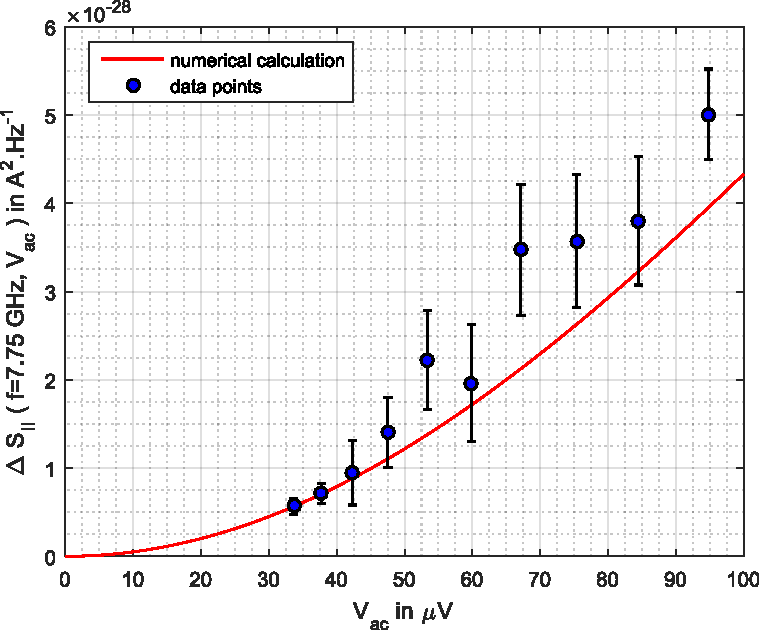
\includegraphics[width = 6.5 cm]{./chap3/RF_noise_vs_pump_amp}
		\end{tabular}
	\end{center}
	
	\caption{\textbf{Noise generated by the pump voltage.} \textbf{(a)} Low frequency noise $\Delta S_{II}\left(f = 0\right)$ as a function of the pump amplitude $V_{\mathrm{ac}}$ with no bias voltage applied $V_{\mathrm{dc}} = 0$ V. The model is numerically calculated by evaluating equation \eqref{eq: LF noise vs pump amp}. \textbf{(b)} High frequency noise $\Delta S_{II}\left(f = 7.75 \mathrm{GHz} \right)$ as a function of the pump amplitude $V_{\mathrm{ac}}$ with no bias voltage applied $V_{\mathrm{dc}} = 0$ V. For these measurements the pump voltage is modulated so the excess noise is the noise difference between pump amplitude $V_{\mathrm{ac}}$ and 0, $\Delta S_{II} = S_{II}\left(V_{\mathrm{ac}}\right)-S_{II}\left(V_{\mathrm{ac}=0}\right)$. The model is evaluated by numerical calculations of the pump Wigner distribution and equations ... .}
	\label{fig: noise pump vs amp}
\end{figure}

The set-up in the lower part of figure ... measures the reduction of the noise of squeezed states but compared to the noise of the RF sinus.
In order to demonstrate a reduction of the noise below the vacuum, the RF sinus noise is measured in this paragraph.
The circuit in the top part of figure ... is chosen with the parameters $V_{\mathrm{dc}}$ equals 0 V and the amplitude of the RF sinus $V_{\mathrm{pump}}$ is varied in a range used in the following measurements.

In the panel (a) of figure \ref{fig: noise pump vs amp}, the low frequency excess noise is plotted as a function of $V_{\mathrm{ac}}$, the attenuated value of $V_{\mathrm{pump}}$ at the quantum point contact location.
This figure is connected to the panel (a) of figure \ref{fig: noise pump vs Vdc} by the point at $V_{\mathrm{dc}} = 0$ V of t\ref{fig: noise pump vs Vdc} is equal to the point at $V_{\mathrm{ac}} = 38$ $\upmu$V of the currently discussed figure \ref{fig: noise pump vs amp} (a).
This measurement enables to calibrate $V_{\mathrm{ac}}$, since the attenuation of RF line carrying $V_{\mathrm{pump}}$ is chosen in order that data points fits the numerically calculated line.
The numerical calculations is based on photo-assisted shot noise formula \ref{eq: LF noise vs pump amp}, and as already demonstrated in previous experiments ... the data points are also in this experiment well distributed on the model.

In the panel (b) the quantity of interest, which is the high frequency noise of a RF sinus, is measured as a function of its amplitude $V_{\mathrm{ac}}$.
The measurements cover approximately the same range for $V_{\mathrm{ac}}$ as in panel (a), and the two values between 30 $\upmu$V and 40 $\upmu$V are more precisely measured because they are the ones used in squeezing measurements. 
In this measurement the phase between the RF sinus pump at 7.75 GHz and the local oscillator at 15.5 GHz does not affect the excess noise.
The real and imaginary parts of the excess noise give the same results and are averaged together on the graph.
The two results $\Delta S_{II} = ... \pm ...$ for $V_{\mathrm{ac}} = 34$ $\upmu$V and $\Delta S_{II} = ... \pm ...$ for $V_{\mathrm{ac}} = 38$ $\upmu$V are used in the following.

\subsection{Phase dependence of noise generated by both DC voltage and RF sinus}

\begin{figure}[hptb]
	\begin{center}
		\begin{tabular}{c}
			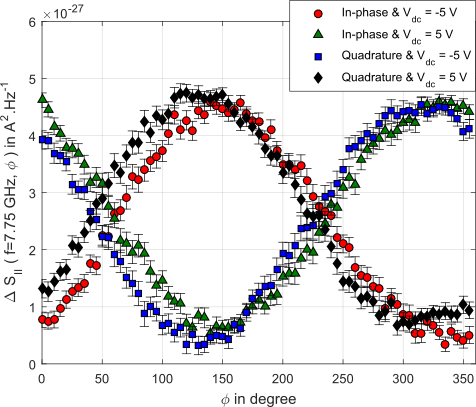
\includegraphics[width = 6.5 cm]{./chap3/RF_noise_vs_pump_phase}
		\end{tabular}
	\end{center}
	
	\caption{\textbf{High frequency noise as a function of pump phase.} The High frequency noise is recorded as a function of the phase difference between the pump and the local oscillator. The two components of the noise are plotted, in red circles and green triangles for in phase components, and in blue squares and black diamonds for quadrature components. For each components two opposite values of bias are applied, a negative bias for red circles and blue squares, and a positive bias for green triangles and black diamonds. The four data set follow a sine curve and the phase of the sine is shifted by $180^{\circ}$ between two different quadratures or two opposite bias.}
	\label{fig: noise pump vs phase}
\end{figure}

In the previous subsection, the high frequency noise generated only by a RF sinus does not depend on the phase difference between the RF sinus and the local oscillator as for the noise generated only by a DC voltage measured in chapter ... .
In the panel (b) of figure Fig.\ref{fig: noise pump vs Vdc}, the noise is generated by both a RF sinus and a DC voltage in this experiment only the difference of noise magnitude are measured but the excess noise is not the simple addition of the contribution of each source.
In this subsection we study the phase dependence of this noise when both RF and DC sources are used, this effect is used in subsection ... to generate and measure a squeezed state.
The set-up used to measure the data points plotted in figure Fig.\ref{fig: noise pump vs phase}, modulate the DC voltage and acquire the real and imaginary parts of the excess noise.
To enhance the effect of the phase dependence, the DC voltage is set at $\pm5$ V at the room temperature source output, which corresponds to approximatively $\pm100$ $\upmu$V applied on the ohmic contact.
The data points are measured every $5^\circ$ of phase values in order to check that the points are placed on a sine function, and two other parameters, the sign of the DC voltage and the real or imaginary component of the excess noise, are changed to check that they are equivalent to a $180^\circ$ phase shift.
The results shown in figure Fig.\ref{fig: noise pump vs phase} follow these trends but with a small asymmetry between the measurements of the real part by the in-phase port and the imaginary part by the quadrature port.  
This measurement allows to calibrate the phase of the local oscillator such that the in-phase noise measurement is minimal for the proper DC voltage.

\subsection{High frequency noise reduction below the noise of a vacuum state}

\begin{figure}[hptb]
	\begin{center}
		\begin{tabular}{c c c c}
			(a) & & (b) & \\
			& 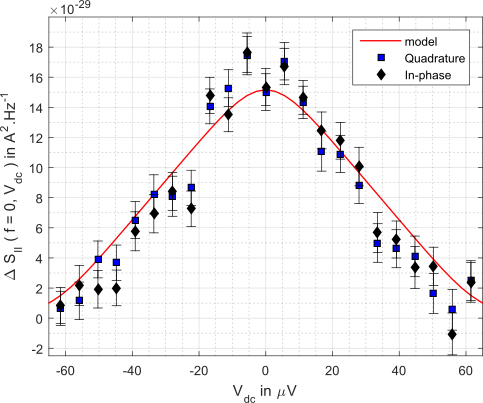
\includegraphics[width = 6.5 cm]{./chap3/LF_noise_squeezed_181206} &
			& 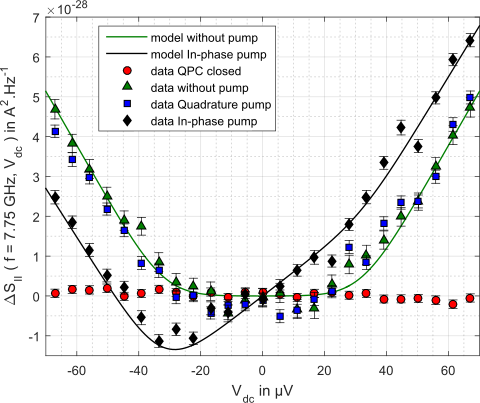
\includegraphics[width = 6.5 cm]{./chap3/RF_noise_squeezed_181206}
		\end{tabular}
	\end{center}
	
	\caption{\textbf{Shot noise as a function of bias voltage with a pump.} \textbf{(a)} Low frequency excess shot noise of the pump is plotted when the pump is in-phase, in black diamond, and in quadrature, in blue square, with the high frequency noise measurement phase reference. The low frequency noise does not depend on the pump phase and they follow the calculated model deduce from the pump Wigner distribution. \textbf{(b)} The high frequency noise is plotted for different parameters of the pump. In red circles the quantum point contact is closed so there is no high frequency noise generated. In green triangles the pump is switched off $V_{\mathrm{ac}} = 0$ V. In blue squares the pump is in quadrature with the noise measurement, the noise measurements are close to the results without pump. In black diamond the pump is in phase with the noise measurement and we measure negative high frequency noise for bias voltage between -20 $\upmu$V and -40 $\upmu$V. Two models are plotted for the high frequency noise without the pump in green line and with the pump in phase in black line.}
	\label{fig: squeezing 181206}
\end{figure}

When the phase of the local oscillator is set thanks to the measurement in the precedent subsection, the DC voltage is swept in a $\pm 60$ $\upmu$V range where the noise reduction is expected.
This subsection explains, with the figure Fig.\ref{fig: squeezing 181206}, the measurement that shows a squeezed state.
The panel (a) of figure Fig.\ref{fig: squeezing 181206}, is a low frequency spectroscopy noise measurement done at the same time as high frequency measurement, and confirms that the amplitude of RF sinus is at $V_{\mathrm{ac}} = 32$ $\upmu$V.
The noise of the RF sinus alone has been precisely measured slightly above this amplitude at $V_{\mathrm{ac}} = 34$ $\upmu$V in previous subsection at $\Delta S_{II} = ...$, so it can be used as a reference and the excess noise is measured compared to this value thanks to the set-up at the bottom part of figure Fig.\ref{fig: set-up chap 3}.
In the panel (b) of figure Fig.\ref{fig: squeezing 181206}, this excess noise is measured for different parameters choices.
The red circles correspond to a choice of central QPC closed, in that situation there is no noise generation even the reference noise is equal to zero.
The green triangles reproduce the measurements of chapter ... in the integer quantum hall regime without RF sinus.
As the experimental set-up measure simultaneously both in-phase and quadrature of the high frequency noise, both measurements are plotted on the graph with blue squares and black diamonds.
The blue squares are the excess noise components which is only the noise of the DC voltage added to the reference noise of the RF pump.
The black diamonds are the measurements which shows the maximal noise variations compared to the DC voltage added noise, and they agree with the model plotted with the black line.
The points for DC voltages between -20 $\upmu$V and -40 $\upmu$V are negatives as expected with the model which means that the noise is smaller than the noise of the RF sinus.
The smallest excess noise value measured is $\Delta S_{II} = ...$, so it is smaller than the noise added to the vacuum by the RF sinus $\Delta S_{II} = ...$, so for smallest excess noise measured the corresponding state is a squeezed state with a component generating less noise than the vacuum state. 

\subsection{Complementary high frequency noise reduction measurements}

\begin{figure}[hptb]
	\begin{center}
		\begin{tabular}{c c c c}
			(a) & & (b) & \\
			& 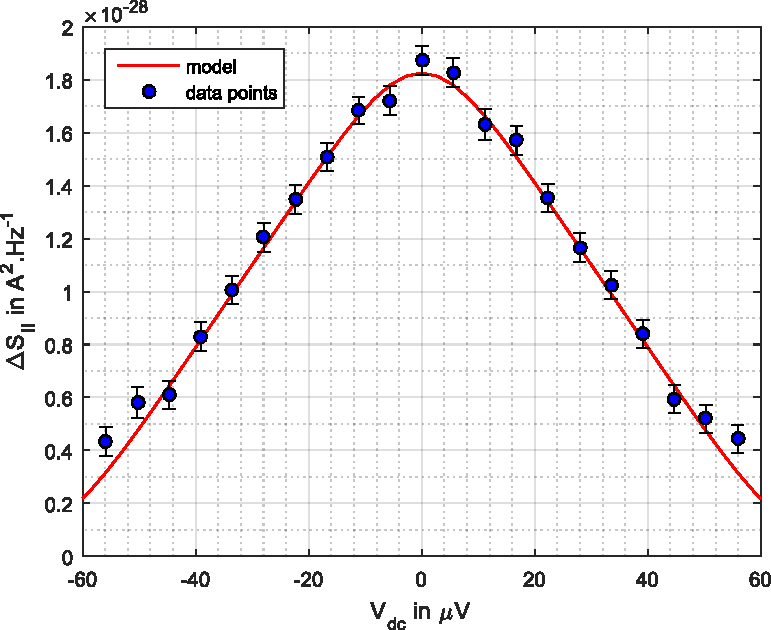
\includegraphics[width = 6.5 cm]{./chap3/LF_noise_squeezed_181112} &
			& 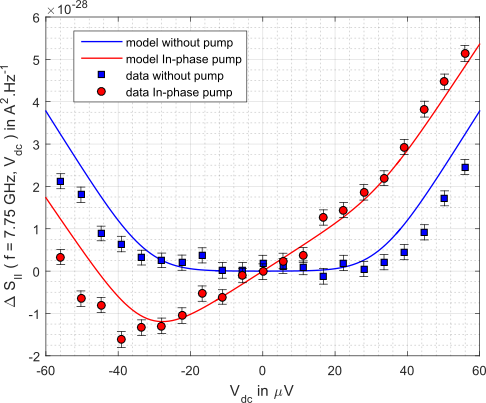
\includegraphics[width = 6.5 cm]{./chap3/RF_noise_squeezed_181112} \\
			(c) & & (d) & \\
			& 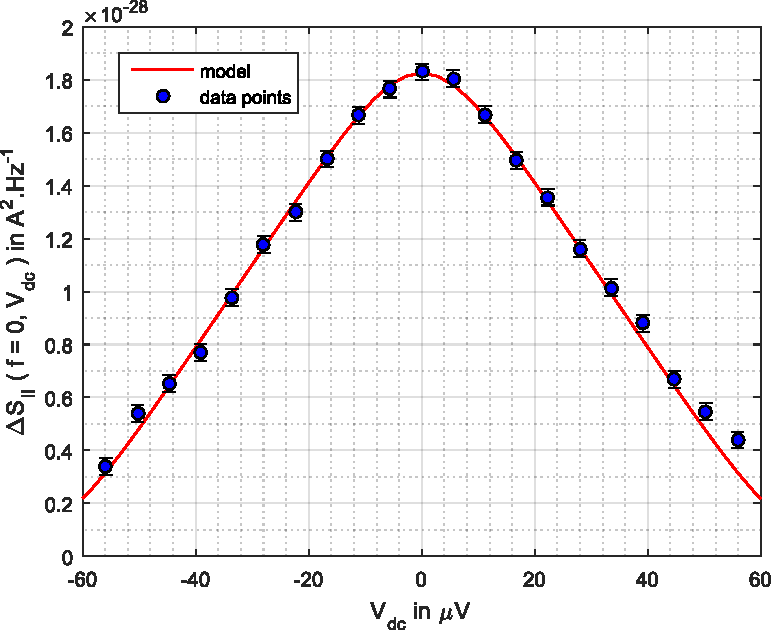
\includegraphics[width = 6.5 cm]{./chap3/LF_noise_squeezed_181108_300mV} &
			& 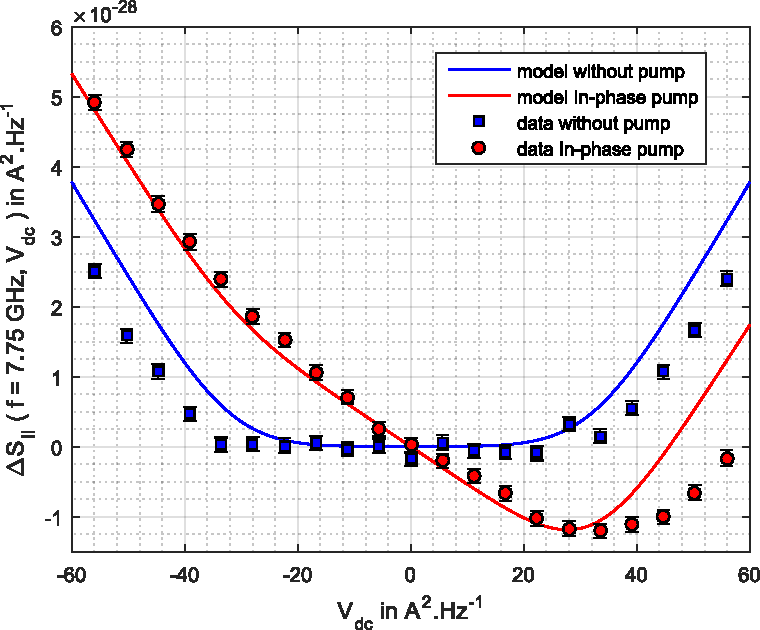
\includegraphics[width = 6.5 cm]{./chap3/RF_noise_squeezed_181108_300mV} \\
			(e) & & (f) & \\
			& 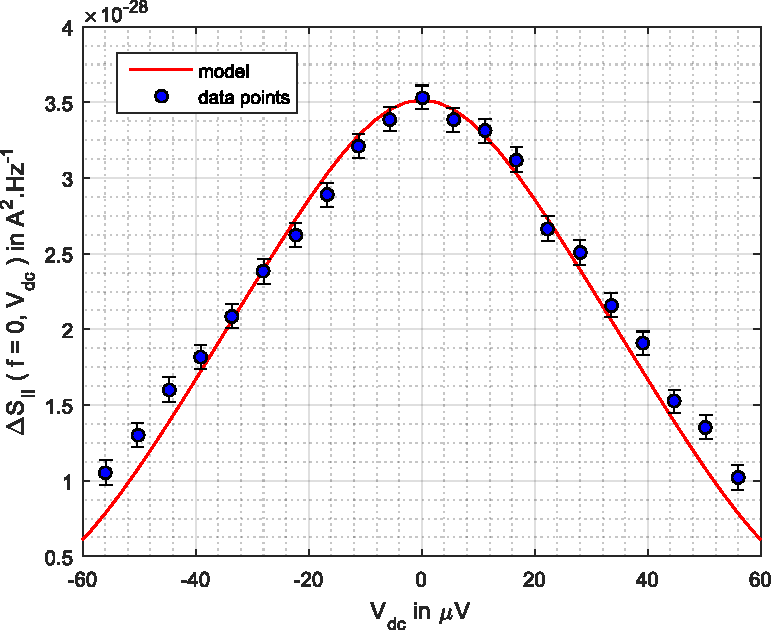
\includegraphics[width = 6.5 cm]{./chap3/LF_noise_squeezed_181108_450mV} &
			& 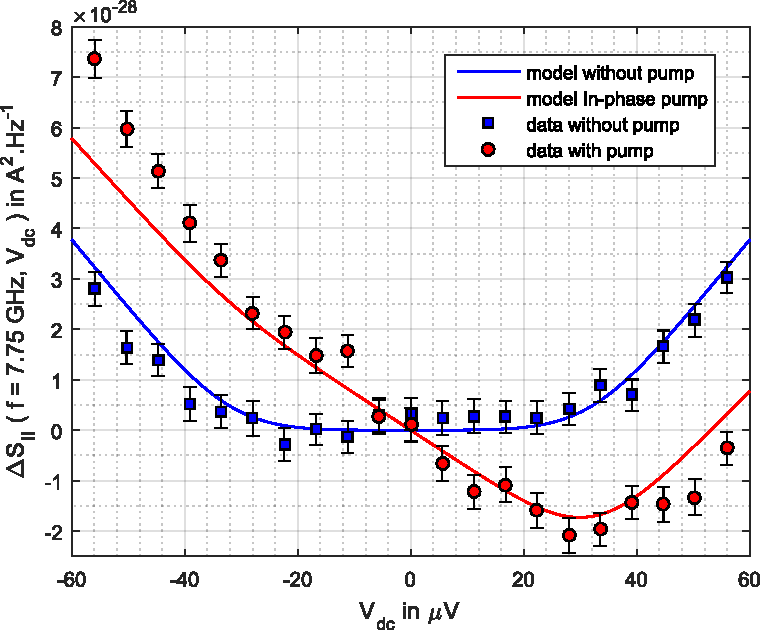
\includegraphics[width = 6.5 cm]{./chap3/RF_noise_squeezed_181108_450mV}
		\end{tabular}
	\end{center}
	
	\caption{\textbf{High frequency noise as a function of bias voltage.} In this graph other measurements of low and high frequency noise are performed with pump voltage of higher amplitude. In panels (a) (c) and (e) the excess low frequency noise of the pump is plotted. In panels (b) (d) (f) the high frequency noise is plotted, in blue square the noise is generated by the DC bias only $V_{\mathrm{ac}} = 0$, in red circles the noise is generated by the DC bias and the pump in phase with phase reference voltages. For each panel on the same line the low frequency noise and high frequency noise are measured simultaneaously, so (a) is paired with (b), (c) with (d), and (e) with (f). The models in red lines are deduce from the Wigner distribution of the pumps and numerical calculations. }
	\label{fig: additional squeezing}
\end{figure}

The measurement of negative high frequency excess noise is repeated for higher amplitude of the RF sinus.
These measurements are summarized in figure Fig.\ref{fig: additional squeezing}, each line of the graph corresponds to one measurement with on the left panel the low frequency noise and on the right panel the high frequency noise. 
Panels (a) and (c) show that panels (b) and (d) have the same RF sinus amplitude $V_{\mathrm{ac}} = 36$ $\upmu$V, the RF sinus have just a phase difference of $\pi$ which explains that negative excess noise appear for positive DC voltage on panel (d).
The noise of a RF sinus alone is measured for a closed amplitude of $V_{\mathrm{ac}} = 38$ $\upmu$V at $\Delta S_{II} = ...$.
On panels (b) and (d) some negative points are placed at $\Delta S_{II} = ...$, so a squeezed state is present at these parameters but some data points do not agree with the model at the edge of the DC voltage range.
The two last panels (e) and (f) show an higher amplitude RF sinus with a low frequency noise of $3.5\times 10^{28}$ A$^2$.Hz$^{-1}$ at zero DC voltage, so its amplitude is around $V_{\mathrm{ac}} = 52$ $\upmu$V thanks to figure Fig.\ref{fig: noise pump vs amp} panel (a).
At this high amplitude the noise of the RF sinus alone has been approximatively measured at $\Delta S_{II} = ...$.
On panel (f) the excess noise is negative and reaches a lowest value of $\Delta S_{II} = ...$, this value is lower than previous high frequency noise but the noise of the RF pump is higher.

\begin{equation}
S_{II}\left(\epsilon\right) = \int_{fc-\Delta f/2}^{fc+\Delta f/2}S_{II}\left(\epsilon,f\right)df
\end{equation}

\begin{equation}
S_{II}\left(\epsilon,f\right) = S_{0}\left(\epsilon,f\right)+S_{pump}\left(\epsilon,f\right)
\end{equation}

\begin{equation}
S_{0}\left(eV,f\right) = 2\frac{e^{2}}{h}k_{B}T\left(\frac{eV-hf}{2k_{B}T}\coth\left(\frac{eV-hf}{2k_{B}T}\right)+\frac{eV+hf}{2k_{B}T}\coth\left(\frac{eV+hf}{2k_{B}T}\right)-\frac{hf}{k_{B}T}\coth\left(\frac{hf}{2k_{B}T}\right)\right)
\end{equation}

\begin{equation}
S_{pump}\left(eV,f\right) = \frac{1}{T}\int_{0}^{T} \left(N\left(eV,hf,t\right)+N\left(eV,-hf,t\right)+2\cos\left(4\pi ft+2\phi\right)N\left(eV,0,t\right)\right)dt
\end{equation}

\begin{equation}
N\left(eV,hf,t\right) = \frac{e^{2}}{h}\int_{-\infty}^{+\infty}g\left(eV,hf,\epsilon\right)\Delta W_{pump}\left(\epsilon,t\right)d\epsilon
\end{equation}

\begin{equation}
g\left(eV,hf,\epsilon\right) = 1-f\left(\epsilon-hf+eV\right)-f\left(\epsilon+hf+eV\right)
\end{equation}

\begin{equation}
\Delta S_{II}\left(f = 0, V_{\mathrm{ac}}\right) = \frac{2e^{2}}{h}\sum_{n = -\infty}^{n = +\infty} J_{n}\left(\frac{eV_{\mathrm{ac}}}{hf}\right)^{2}nhf\coth\left(\frac{nhf}{2k_{\mathrm{B}}T_{\mathrm{elec}}}\right)-4\frac{e^{2}}{h}k_{\mathrm{B}}T_{\mathrm{elec}} \label{eq: LF noise vs pump amp}
\end{equation}

where $J_{n}$ are Bessel functions.


%\begin{figure}[hptb]
%	\begin{center}
%		\begin{tabular}{c c c c}
%			(a) & & (b) & \\
%			& 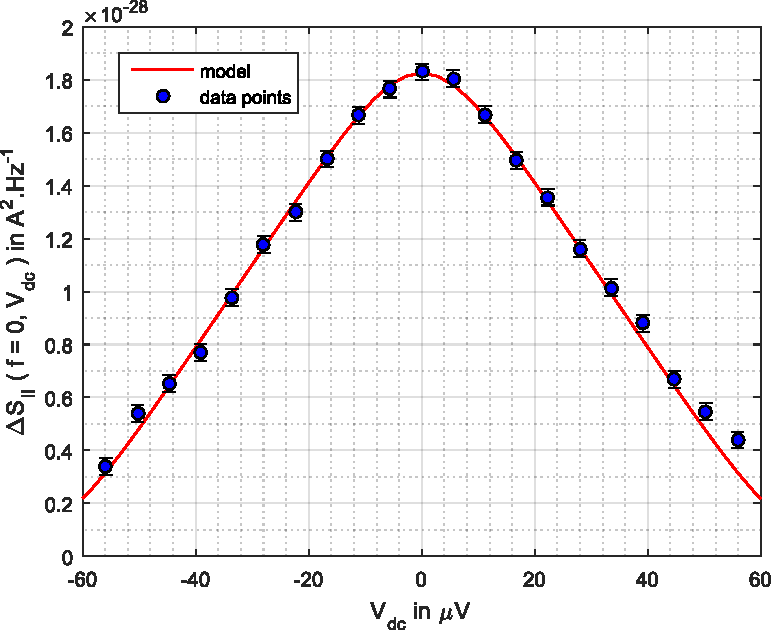
\includegraphics[width = 6.5 cm]{./chap3/LF_noise_squeezed_181108_300mV} &
%			& 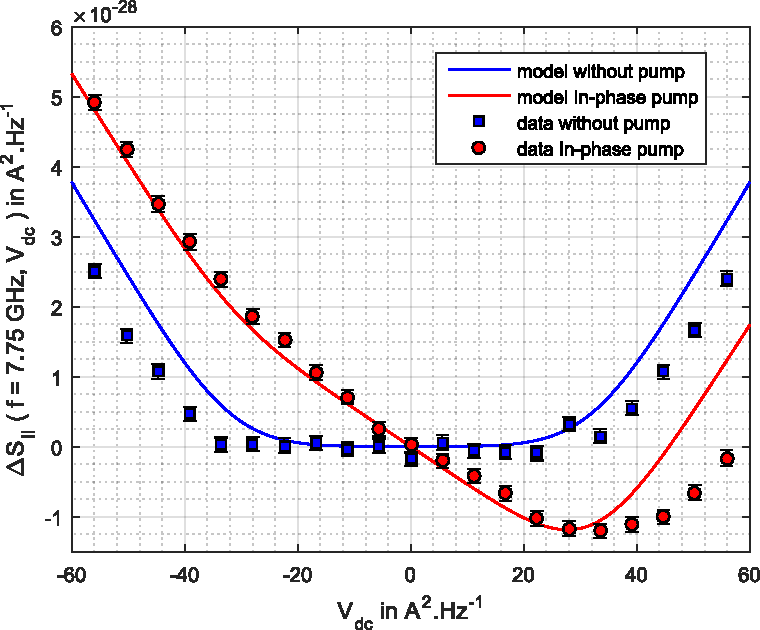
\includegraphics[width = 6.5 cm]{./chap3/RF_noise_squeezed_181108_300mV}
%		\end{tabular}
%	\end{center}
%	
%	\caption{\textbf{High frequency noise as a function of bias voltage.}}
%	\label{fig: squeezing 181108 300mV}
%\end{figure}

%\begin{figure}[hptb]
%	\begin{center}
%		\begin{tabular}{c c c c}
%			(a) & & (b) & \\
%			& 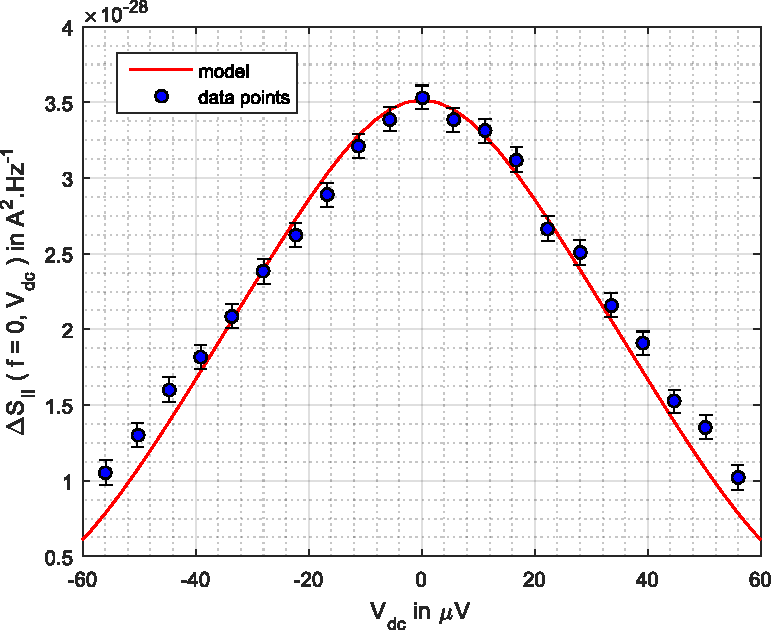
\includegraphics[width = 6.5 cm]{./chap3/LF_noise_squeezed_181108_450mV} &
%			& 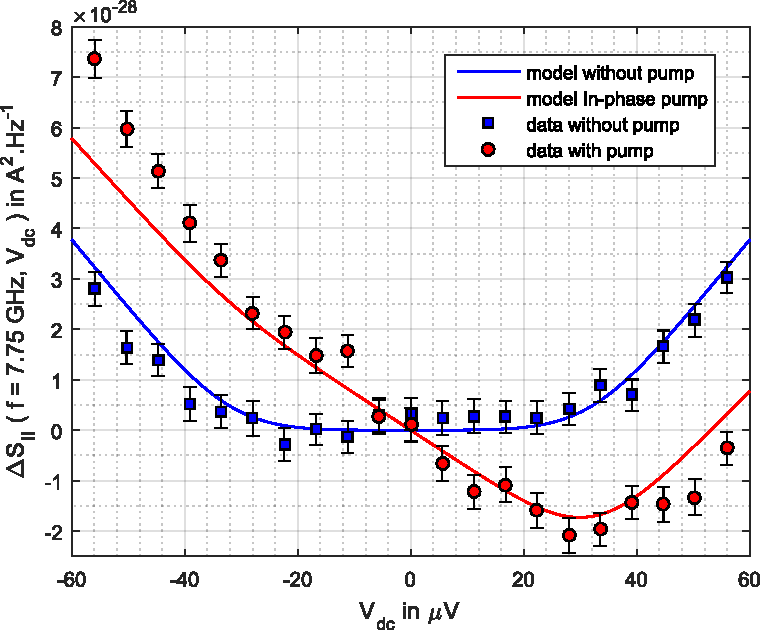
\includegraphics[width = 6.5 cm]{./chap3/RF_noise_squeezed_181108_450mV}
%		\end{tabular}
%	\end{center}
%	
%	\caption{\textbf{High frequency noise as a function of bias voltage.}}
%	\label{fig: squeezing 181108 450mV}
%\end{figure}

%\begin{enumerate}
%	\item simu avec aspect électronique Wigner
%	\item simu avec aspect bosons
%	\item mesure de bruit RF
%	\item interprétation en terme de squeezing
%\end{enumerate}

%\section{\texorpdfstring{Description avec edge-magnetoplasmon}{}}

%\section{\texorpdfstring{Calculs du squeezing avec aspects electron/bosons}{}}

%\section{\texorpdfstring{Comment on le mesure avec bruit RF}{}}

%\section{\texorpdfstring{Résultats en terme de squeezing}{}}